\section{Auswertung}
\label{sec:Auswertung}

\subsection{Schwellenstrom}
\label{subsec:Schwellenstrom}
Zur Auswertung des Schwellenstromes des Diodenlasers wird der Strom langsam aufgedreht, bis die charakteristische Lasergranulation auftritt. Im Versuch
ergab sich ein Schwellenstrom von $\SI{34,4}{\milli\ampere}$. \newline
Es wurden drei Fotografien des Displays der Infrarotkamera gemacht, die in \autoref{fig:Aufnahmen} abgebildet sind.

\begin{figure}[H]
  \centering
  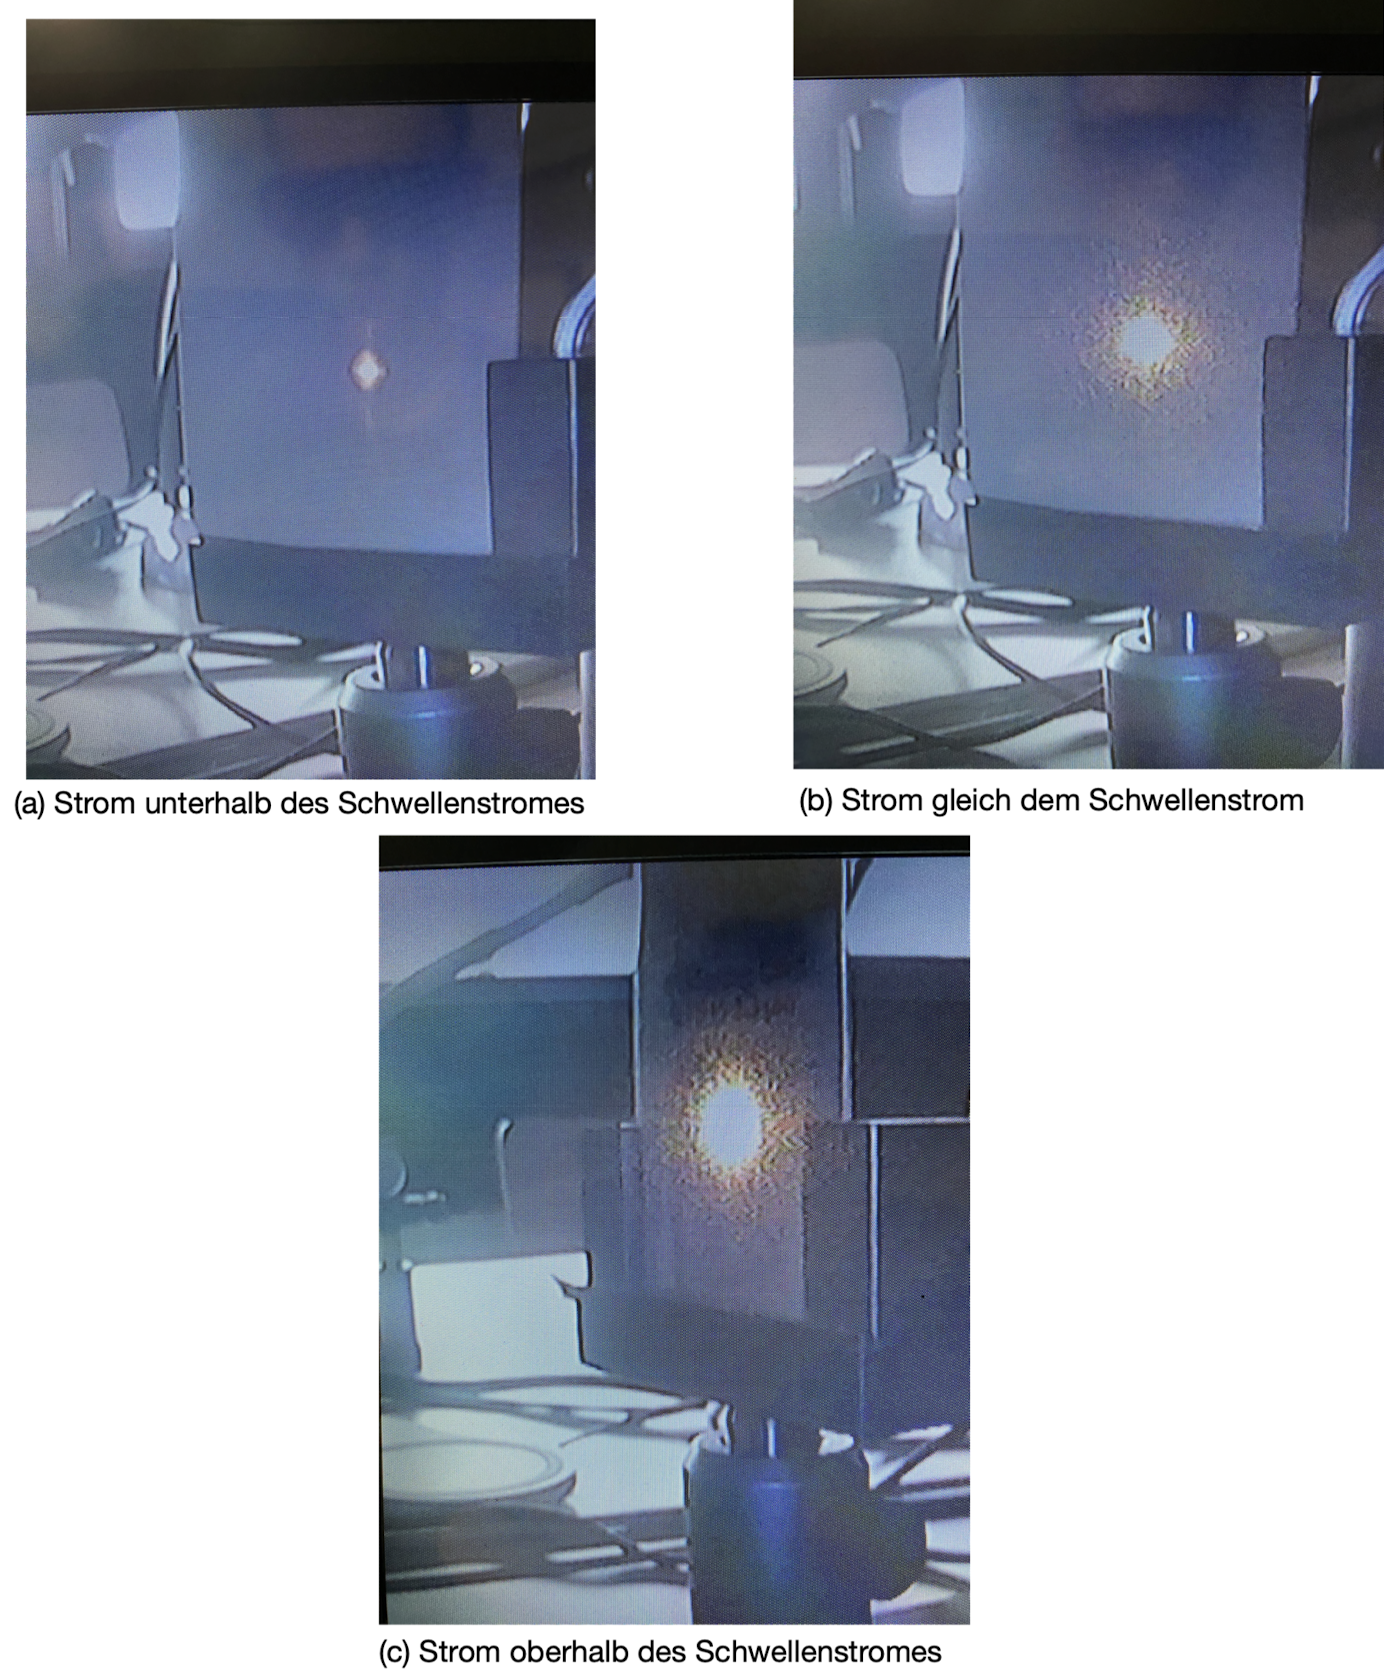
\includegraphics[width=0.68\textwidth]{data/Aufnahmen.png}
  \caption{Fotografie des Displays der Infrarotkamera bei unterschiedlichen Strömen.}
  \label{fig:Aufnahmen}
\end{figure}

\subsection{Rubidiumfluoreszenz}
\label{subsec:Rubidiumfluoreszenz}

Wird der Laser auf das mit Rubidium gefüllte Gefäß gerichtet, kann die Rubidiumfluoreszenz beobachtet werden. Zur Auswertung wurde mit der Infrarotkamera ein Bild der Fluoreszenz aufgenommen und
in \autoref{fig:fluoreszenz} dargestellt. Es ist eine gelbliche Linie zu erkennen, die durch die Rubidiumatome erzeugt wird, wenn sie innerhalb des Gefäßes mit dem Laser fluoreszieren.

\begin{figure}[H]
  \centering
  \includegraphics[width=0.5\textwidth]{data/Fluoreszenz.png}
  \caption{Fotografie des Displays der Infrarotkamera der Rubidiumfluoreszenz.}
  \label{fig:fluoreszenz}
\end{figure}

\subsection{Transmissionsspektrum}
\label{subsec:Transmissionsspektrum}

Zur Auswertung des Transmissionsspektrums von Rubidium wurde in \autoref{fig:spektrum} eine Fotografie des Oszilloskopes erstellt, die das Transmissionsspektrum von Rubidium zeigt.

\begin{figure}[H]
  \centering
  \includegraphics[width=0.7\textwidth]{data/spektrum.png}
  \caption{Fotografie des Transmissionsspektrums von Rubidium.}
  \label{fig:spektrum}
\end{figure}